%%%%%%%%%%%%%%%%%%%%%%%%%%%%%%%%%%%%%%%%%
% Beamer Presentation
% LaTeX Template
% Version 1.0 (10/11/12)
%
% This template has been downloaded from:
% http://www.LaTeXTemplates.com
%
% License:
% CC BY-NC-SA 3.0 (http://creativecommons.org/licenses/by-nc-sa/3.0/)
%
%%%%%%%%%%%%%%%%%%%%%%%%%%%%%%%%%%%%%%%%%

%----------------------------------------------------------------------------------------
%	PACKAGES AND THEMES
%----------------------------------------------------------------------------------------

\documentclass{beamer}

\mode<presentation> {

% The Beamer class comes with a number of default slide themes
% which change the colors and layouts of slides. Below this is a list
% of all the themes, uncomment each in turn to see what they look like.

%\usetheme{default}
%\usetheme{AnnArbor}
%\usetheme{Antibes}
%\usetheme{Bergen}
%\usetheme{Berkeley}
%\usetheme{Berlin}
%\usetheme{Boadilla}
%\usetheme{CambridgeUS}
%\usetheme{Copenhagen}
%\usetheme{Darmstadt}
%\usetheme{Dresden}
%\usetheme{Frankfurt}
%\usetheme{Goettingen}
%\usetheme{Hannover}
%\usetheme{Ilmenau}
%\usetheme{JuanLesPins}
%\usetheme{Luebeck}
\usetheme{Madrid}
%\usetheme{Malmoe}
%\usetheme{Marburg}
%\usetheme{Montpellier}
%\usetheme{PaloAlto}
%\usetheme{Pittsburgh}
%\usetheme{Rochester}
%\usetheme{Singapore}
%\usetheme{Szeged}
%\usetheme{Warsaw}

% As well as themes, the Beamer class has a number of color themes
% for any slide theme. Uncomment each of these in turn to see how it
% changes the colors of your current slide theme.

%\usecolortheme{albatross}
%\usecolortheme{beaver}
%\usecolortheme{beetle}
%\usecolortheme{crane}
%\usecolortheme{dolphin}
%\usecolortheme{dove}
%\usecolortheme{fly}
%\usecolortheme{lily}
%\usecolortheme{orchid}
%\usecolortheme{rose}
%\usecolortheme{seagull}
%\usecolortheme{seahorse}
%\usecolortheme{whale}
%\usecolortheme{wolverine}

%\setbeamertemplate{footline} % To remove the footer line in all slides uncomment this line
%\setbeamertemplate{footline}[page number] % To replace the footer line in all slides with a simple slide count uncomment this line

\setbeamertemplate{navigation symbols}{} % To remove the navigation symbols from the bottom of all slides uncomment this line
}

\usepackage{graphicx} % Allows including images
%\usepackage{booktabs} % Allows the use of \toprule, \midrule and
                      % \bottomrule in tables
\usepackage{tikz}
\usepackage{tikz-cd}
\usepackage{varwidth}
\usepackage{amsmath}
\usepackage[author-year]{amsrefs}
\usepackage{../ReAdTeX/readtex-core}
% \usepackage{../ReAdTeX/readtex-dangerous}
% \usepackage{../ReAdTeX/readtex-abstract-algebra}
\usepackage{ytableau}
%%%%%%%%%%%%%%%%%%%%%%%%%%%%%%%%%%%%%%%%%%%%%%%%%%%%%%%%%%%%%%%%%%% 
%%  MACRO DEFINITIONS:  Co-authors -- PLEASE use these! 
%%%%%%%%%%%%%%%%%%%%%%%%%%%%%%%%%%%%%%%%%%%%%%%%%%%%%%%%%%%%%%%%%%%
\definecolor{coralred}{rgb}{1.0, 0.25, 0.25}
\definecolor{lightblue}{rgb}{.3,.65,1.0} %
\DeclareMathOperator{\Gr}{Gr}
\newcommand{\cupprod}{\cup}
\newcommand{\sym}{\Lambda}
\newcommand{\lowers}{\mathcal{L}}
\newcommand{\mynone}{\ }
\newcommand{\G}{\mathfrak{G}}
\renewcommand{\S}{\mathfrak{S}}

%%%%%%%%%%%%%%%%%%%%%%%%%%%%%%%%%%%%%%%%%%%%%%%%%%%%%%%%%%%%%%%%%%%% 


%----------------------------------------------------------------------------------------
%	TITLE PAGE
%----------------------------------------------------------------------------------------

\title[\(K\)-theory Catalans]{\(K\)-theoretic Catalan functions} % The short title appears at the bottom of every slide, the full title is only on the title page

\author[George H. Seelinger]{George H. Seelinger (joint with
  J. Blasiak and J. Morse)} % Your name
\institute[UVA] % Your institution as it will appear on the bottom of every slide, may be shorthand to save space
{
CAGE \\ % Your institution for the title page
\medskip
\textit{ghs9ae@virginia.edu} % Your email address
}
\date{6 February 2020} % Date, can be changed to a custom date

\begin{document}

\begin{frame}
\titlepage % Print the title page as the first slide
\end{frame}
% \begin{frame}[fragile]{Overview}
%   \begin{enumerate}
%   \item An overview of Schubert calculus
%   \item An interlude: Catalan functions
%   \item Toward the \(K\)-theory and \(K\)-homology of the affine
%     Grassmannian
%     \[
%       \begin{tikzcd}
%         H(\Gr(m,n)) \ar[d] \ar[r]& H(\Gr_{SL_{k+1}}) \ar[d] \\
%         K(\Gr(m,n)) \ar[r] & K(\Gr_{SL_{k+1}})
%       \end{tikzcd}
%     \]
%   \item A resolution: \(K\)-theoretic Catalan functions
%   \end{enumerate}
% \end{frame}
\begin{frame}{Overview}
  \begin{itemize}
  \item Schubert calculus
  \item Catalan functions: a new approach to old problems
  \item \(K\)-theoretic Catalan functions
  \end{itemize}
\end{frame}
\begin{frame}{Overview of Schubert Calculus Combinatorics}
  \begin{block}{Geometric problem}
    Find \(c_{\lambda \mu}^\nu = \#\) of points in
    intersection of subvarieties in a variety \(X\). \pause
  \end{block}
  \[
    \downarrow
  \]
  \begin{block}{Cohomology}
    Schubert basis \(\{\sigma_\lambda\}\) for \(H^*(X)\) with property \(\sigma_\lambda \cupprod \sigma_\mu = \sum_\nu c_{\lambda \mu}^\nu \sigma_\nu\) \pause 
\end{block}
\[
  \downarrow
\]
\begin{block}{Representatives}
  Special basis of polynomials \(\{f_\lambda\}\) such that \(f_\lambda \cdot f_\mu = \sum_\nu c_{\lambda \mu}^\nu f_\nu\)
\end{block}
\end{frame}
\begin{frame}{Overview of Schubert Calculus Combinatorics (cont.)}
  Combinatorial study of \(\{f_\lambda\}\) enlightens the geometry
  (and cohomology). %\pause
  \begin{alertblock}{Goal}
    Identify \(\{f_\lambda\}\) in explicit (simple) terms amenable to
    calculation and proofs.
  \end{alertblock}
\end{frame}
% \begin{frame}{Classical Example}
%   \(X = \Gr_m(\C^{m+n}) = \{\text{all }m\text{-dimensional subspaces of
%   }\C^{n+m}\}\). 

%   Decomposes into Schubert varieties indexed by partitions \(\lambda \subset (\underbrace{n,
%     \ldots, n}_{m}) = (n^m)\). \[
%     \ytableausetup{boxsize=0.5em}
%     \ydiagram[*(gray)]{3,3} \quad
%     \ydiagram{3,3}*[*(gray)]{2,3} \quad
%     \ydiagram{3,3}*[*(gray)]{2,2} \quad
%     \ydiagram{3,3}*[*(gray)]{1,3} \quad
%     \ydiagram{3,3}*[*(gray)]{0,3} \quad
%     \ydiagram{3,3}*[*(gray)]{1,2} \quad
%     \ydiagram{3,3}*[*(gray)]{1,1} \quad
%     \ydiagram{3,3}*[*(gray)]{0,2} \quad
%     \ydiagram{3,3}*[*(gray)]{0,1} \quad
%     \ydiagram{3,3}
%   \]
%   \begin{itemize}
%   \item \(H^*(\Gr_m(\C^{m+n})) = \bigoplus_{\lambda \subset (n^m)} \Z
%     \sigma_\lambda\) as \(\Z\)-modules
%   \item \(\sigma_\lambda \cupprod \sigma_\mu = \sum_\nu c_{\lambda
%       \mu}^\nu \sigma_\nu\)
%   \end{itemize}
%   \(c_{\lambda \mu}^\nu = \)number of points in intersection of
%   Schubert varieties.

%   What are the structure constants \(c_{\lambda \mu}^\nu\)?
% %   \begin{example}
% %     \begin{itemize}
% %     \item \(X = \Gr_{m,n}\) %\pause
% %     \item \(f_\lambda = s_\lambda\), the Schur functions %\pause
% %     \item \(s_\lambda = \prod_{i < j} (1-R_{ij})h_\lambda\)
% %       (Jacobi-Trudi) %\pause
% %       \item Raising operators
% %     \(R_{i,j}(h_\lambda) = h_{\lambda+\epsilon_i-\epsilon_j}\)
% %     \ytableausetup{boxsize=0.5em}
% %     \[
% %       R_{1,3} \left( \ydiagram{1,1,3}*[*(red)]{1} \right) =
% %       \ydiagram{1,4}*[*(red)]{0,3+1} \ \ \ R_{2,3} \left(
% %         \ydiagram{1,1,1}*[*(red)]{1} \right) =
% %       \ydiagram{2,1}*[*(red)]{1+1}
% %     \] 
% % %    %\pause
% % %    \item Structure constants are determined by the Pieri rule: \(h_r s_\lambda = \sum_{\mu} s_\mu\)
% %     \end{itemize}
% %   \end{example}
% \end{frame}
% \begin{frame}{Classical Example (cont.)}
%   \(\sym_m = \C[x_1, \ldots, x_m]^{S_m}\) is the ring of symmetric
%   polynomials in \(m\) variables and has bases indexed by partitions.

%   \begin{center}
%     \(\underbrace{12 x_1^2 + 12 x_2^2 - 7 x_1
%       x_2}_{\text{symmetric}}\) \ \ \ \ \
%     \(\underbrace{5 x_1^2 + 12 x_2^2 - 7 x_1 x_2}_{\text{not
%         symmetric}}\)
%   \end{center}
%   There exists a basis of \(\sym_m\) denoted \(\{s_\lambda\}_\lambda\)
%   and a surjection of rings such that
%   \begin{align*}
%     \sym_m
%     & \to H^*(\Gr(m,n)) \\
%     s_\lambda
%     & \mapsto
%       \begin{cases}
%         \sigma_\lambda & \lambda \subset (n^m) \\
%         0 & \text{otherwise.}
%       \end{cases}
%   \end{align*}
% \end{frame}
% \begin{frame}{Classical Example (cont.)}
%   Cohomology structure: \(\sigma_\lambda \correspondsto
%   s_\lambda\) when \(\lambda \subset (n^m)\). \[
%     s_\lambda s_\mu = \sum_{\nu \subset (n^m)} \textcolor{blue}{c_{\lambda \mu}^\nu}
%     s_\nu + \sum_{\nu \not\subset (n^m)} \textcolor{red}{c_{\lambda \mu}^\nu} s_\nu
%     \correspondsto \sigma_\lambda \cupprod \sigma_\mu =
%     \sum_{\nu \subset (n^m)} \textcolor{blue}{c_{\lambda \mu}^\nu} \sigma_\nu
%   \]
% \end{frame}
% \begin{frame}{Schur functions \(s_\lambda\)}
%   \ytableausetup{boxsize=1.0em}
%   \begin{example}
%     \emph{Semistandard tableaux}: columns increasing and rows non-decreasing.\[
%       \ytableaushort{5,34,23,1225} \ \ \ \
%       \underbrace{\ytableaushort{8,79,34,1256}}_{\text{standard = no
%           repeated letters}}
%     \]
%   \end{example}
%   Schur function \(s_\lambda\) is a ``weight generating function'' of
%   semistandard tableaux:
%   \begin{align*}
%       \ytableausetup{boxsize=1.0em,aligntableaux=bottom}
%     & \ytableaushort{2,11},\  \ytableaushort{3,11},\ \ytableaushort{3,22},\
%     \ytableaushort{2,12},\ \ytableaushort{3,13},\ \ytableaushort{3,23},\
%     \ytableaushort{2,13},\ \ytableaushort{3,12}\\
%     \ytableausetup{boxsize=0.3em}
%     s_{\ydiagram{1,2}}(x_1,x_2,x_3) = & x_1^2x_2+x_1^2x_3+x_2^2x_3+x_1x_2^2+x_1x_3^2+x_2x_3^2+2x_1x_2x_3
%   \end{align*}
% \end{frame}
% \begin{frame}{Schur functions \(s_\lambda\) (cont.)}
%   \begin{block}{Pieri rule}
%     Determines multiplicative structure: \[
%       s_r s_\lambda = \sum (1 \text{ or }0) s_\nu 
%     \] \[
%       s_{\ydiagram{1}} s_{\ydiagram{1,2}} =
%       s_{\ydiagram{1,3}*[*(red)]{0,2+1}} +
%       s_{\ydiagram{2,2}*[*(red)]{1+1}} + s_{\ydiagram{1,1,2}*[*(red)]{1}}
%     \]
%   \end{block}
%   Iterate Pieri rule \[
%     s_{\mu_1} \cdots s_{\mu_r} s_\lambda = \sum (\# \text{ known
%       tableaux})s_\nu
%   \]
%   Since \(s_{\mu_1} \cdots s_{\mu_r} = s_{(\mu_1, \ldots, \mu_r)} +\)
%   lower order terms, subtract to get \[
%     s_{(\mu_1, \ldots, \mu_r)} s_\lambda = \sum c_{\lambda \mu}^\nu s_\nu
%   \]
%   for well-understood \emph{Littlewood-Richardson coefficients}
%   \(c_{\lambda \mu}^\nu\). 
% \end{frame}
\begin{frame}{Classical Schubert Calculus}
    \begin{block}{Geometric problem}
    Find \(c_{\lambda \mu}^\nu = \#\) of points in
    intersection of Schubert varieties \(\{X_\lambda\}_{\lambda
      \subset (n^m)}\) in variety \(X = \Gr(m,n)\). \pause
  \end{block}
  \vspace{-0.1in}
  \[
    \downarrow
  \]
  \vspace{-0.1in}
  \begin{block}{Cohomology}
    Schubert basis \(\{\sigma_\lambda\}_{\lambda \subset (n^m)}\) for \(H^*(X)\) with property \(\sigma_\lambda \cupprod \sigma_\mu = \sum_\nu c_{\lambda \mu}^\nu \sigma_\nu\) %\pause 
  \end{block}\pause
\vspace{-0.1in}  
\[
  \downarrow
\]
\vspace{-0.1in}
\begin{block}{Representatives}
  Special basis of Schur polynomials \(\{s_\lambda\}\) such that
  \(s_\lambda \cdot s_\mu = \sum_\nu c_{\lambda \mu}^\nu s_\nu\) for
  Littlewood-Richardson coefficients \(c_{\lambda \mu}^\nu\).
\end{block}
\end{frame}
\begin{frame}{Next Step: Flag Variety}
  \begin{itemize}
  \item
    \(X = Fl_n(\C) = \{V_0 \subset V_1 \subset \cdots \subset
    V_n \st \dim V_i = i\}\) \pause

   \item Decomposes into Schubert varieties indexed by \(w \in S_n\).\pause

    \item \(H^*(Fl_n(\C))\) supported by Schubert polynomials
    \(\S_w \in \Z[x_1, \ldots, x_n]\) (Not necessarily symmetric!) \pause
  \end{itemize}
  \begin{block}{Open Problem}
    Structure constants \(\S_w \S_u = c_{w u}^v \S_v \) are
    combinatorially unknown.
  \end{block}
\end{frame}
\begin{frame}[fragile]{Schubert Calculus Variations}
    There are many variations on classical Schubert calculus of
    the Grassmannian (Type A).
    \pause
    \begin{tabular}{|c|c|}
      \hline
      Theory
      & \(f_\lambda\) \\
      \hline
      (Co)homology of Grassmannian
      & Schur functions\\
      \hline
      (Co)homology of flag variety
      & Schubert polynomimals\\
      \hline
      Quantum cohomology of flag variety
      & Quantum Schuberts\\
      \hline
      (Co)homology of Types BCD Grassmannian
      & Schur-\(P\) and \(Q\) functions\\
      \hline
      (Co)homology of affine Grassmannian
      & (dual) \(k\)-Schur functions\\
      \hline
      \(K\)-theory of Grassmannian
      & Grothendieck polynomials\\
      \hline
      \(K\)-homology of affine Grassmannian
      & \(K\)-\(k\)-Schur functions \\
      \hline
    \end{tabular}
    \pause And many more!
  % \begin{itemize}
  % \item (Co)homology of Types BCD Grassmannian
  % \item \(K\)-theory of Grassmannian
  % \item (Co)homology of affine Grassmannian \(\Gr_{SL_{k+1}} = SL_{k+1}(\C((t)))/SL_{k+1}(\C[[t]])\)
  %   \begin{block}{Goal}
  %     Understand \(K\)-theory and \(K\)-homology of \(\Gr_{SL_{k+1}}\).
  %   \end{block}
  % \item Simultaneously generalizes \(K\)-theory of Grassmannian and
  %   (co)homology of affine Grassmannian:
  %   \[
  %     \begin{tikzcd}
  %       H(\Gr(m,n)) \ar[d] \ar[r]& H(\Gr_{SL_{k+1}}) \ar[d] \\
  %       K(\Gr(m,n)) \ar[r] & K(\Gr_{SL_{k+1}})
  %     \end{tikzcd} 
  %   \]
  % \end{itemize}
\end{frame}
% \begin{frame}{(Co)homology of Affine Grassmannian}
%   It is known that
%   \begin{itemize}
%   \item  \( H_*(\Gr_{SL_{k+1}}) \isom \Z[s_1, \ldots, s_k]\) 
%   \item \(H^*(\Gr_{SL_{k+1}}) \isom \sym / \langle m_\lambda : \lambda_1 >
%     k\rangle \text{ (Hopf dual) }\)
%   \item Schubert classes in \(H_*(\Gr_{SL_{k+1}})\) correspond to
%     \(k\)-Schur functions \((t=1)\). 
%   \end{itemize}
% \end{frame}
% \begin{frame}{\(k\)-Schur functions and homology of Affine Grassmannian}
%   Denoted \(s_\lambda^{(k)}\) for \(\lambda\) a partition such that
%   \(\lambda_1 \leq k\), \(k\)-Schur functions have equivalent combinatorial
%   descriptions as 
%   \begin{itemize}
%   \item satisfying a Pieri rule based on the weak order of type \(A\)
%     affine Weyl group,
%   \item a weight generating functions over marked chains in the Bruhat
%     order on type \(A\) affine Weyl group,
%   \item a specialization of a broad family of symmetric functions
%     known as Catalan functions.
%   \end{itemize}
%   \begin{block}{Historical Remark}
%     \(k\)-Schur functions with a parameter \(t\) were originally
%     introduced to understand the Schur positivity of Macdonald
%     polynomials. Later,~\cite{Lam} identified them as homology Schubert
%     representatives for the affine Grassmannian when \(t=1\).
%   \end{block}
% \end{frame}
\begin{frame}{Peterson Isomorphism}
  \begin{itemize}
  \item \(QH^*(Fl_{k+1})\) quantum deformation of
    \(H^*(Fl_{k+1})\).\pause
  \item Supported by quantum Schubert polynomials \(\S_w^Q\).\pause
  \item Peterson isomorphism
    \begin{align*}
      \Phi\colon QH^*(Fl_{k+1}) & \to H_*(Gr_{SL_{k+1}})_{loc}\\
      \S_w^Q & \mapsto \frac{s_\lambda^{(k)} }{\prod_{i \in Des(w)} \tau_i} 
    \end{align*}
    where \(s_\lambda^{(k)}\) is a \(k\)-Schur function.
    \pause
  \end{itemize}
  \begin{block}{Upshot}
    Computations for (quantum) Schubert polynomials can be moved into symmetric functions.
  \end{block}
\end{frame}
\begin{frame}{\(k\)-Schur functions}
  \begin{itemize}
  \item \(s_\lambda^{(k)}\) for \(\lambda_1 \leq k\) a basis for
    \(\Z[s_1, s_2, \ldots, s_k]\)~\cite{lapointe-lascoux-morse}. \pause
  \item Schubert representatives for \(H_*(Gr_{SL_{k+1}})\)~\cite{Lam08}. \pause
  \item Has a tableaux formulation and Pieri rule: \(s_{1^r}
    s_\lambda^{(k)} = \sum_{\mu} a_{\lambda \mu} s_\mu^{(k)}\) \pause
  \item \(s_\lambda^{(k)} = s_\lambda\) as \(k \to \infty\).\pause
  \item Branching with positive coefficients~\cite{llms}:
    \ytableausetup{boxsize=0.5em}
      \[s_{\ydiagram{2,2}}^{(2)} =
        \underbrace{s_{\ydiagram{2,2}}}_{s^{(3)}_{\ydiagram{2,2}}}+\underbrace{s_{\ydiagram{1,3}}+s_{\ydiagram{4}}}_{s_{\ydiagram{1,3}}^{(3)}}\] \pause
      \begin{itemize}
      \item Has geometric interpretation.\pause     
      \item No combinatorial interpretation of branching coefficients.\pause
      \item Definition with \(t\) important for Macdonald polynomials.\pause
      \end{itemize}
   \item Many definitions. A new one makes proofs easier!
  \end{itemize}
\end{frame}
\begin{frame}{Overview}
  \begin{itemize}
  \item Schubert calculus
  \item \textbf{Catalan functions: a new approach to old problems}
  \item \(K\)-theoretic Catalan functions
  \end{itemize}
\end{frame}
\begin{frame}{Raising Operators on Symmetric Functions}
  \begin{itemize}
  \item Raising operators \(R_{i,j}\) act on diagrams \[
      \ytableausetup{boxsize=1em,centertableaux}
      R_{1,3} \left( \ydiagram{1,1,3}*[*(red)]{1} \right) =
      \ydiagram{1,4}*[*(red)]{0,3+1} \ \ \ R_{2,3} \left(
        \ydiagram{1,1,1}*[*(red)]{1} \right) =
      \ydiagram{2,1}*[*(red)]{1+1}
    \]\pause
  \item Extend action to a symmetric function \(f_\lambda\) by
    \(R_{i,j}(f_\lambda) = f_{\lambda+\epsilon_i-\epsilon_j}\). \pause
  \item For \(h_\lambda = s_{\lambda_1} \cdots s_{\lambda_r}\), we
    have the \emph{Jacobi-Trudi identity}\[
      s_\lambda = \prod_{i < j} (1-R_{ij}) h_\lambda
    \]\pause
  \end{itemize}
  \begin{align*}
    s_{22} & = (1-R_{12}) h_{22} =  h_{22} - h_{31}\\
    s_{211}
    & = (1-R_{12})(1-R_{23})(1-R_{13}) h_{211}\\
    & = h_{211} - h_{301} - h_{220}\, \textcolor{red}{- h_{310}
      +  h_{310}} + \underbrace{h_{32\,\text{-}1}}_{=0}+h_{400} -  \underbrace{h_{41\,\text{-}1}}_{=0}
  \end{align*}
  \textcolor{red}{some terms cancel}
\end{frame}
\begin{frame}{Raising Operators on Symmetric Functions}
  Gives definition for Schur function indexed by any
  integer vector \(\alpha \in \Z^\ell\). \pause Straightening: \[
s_\alpha = \prod_{i<j} (1-R_{ij}) h_\alpha = 
\begin{cases} \pm\, s_\lambda & \text{for a partition $\lambda$} \\0\end{cases}
\]
\pause For \(\langle s_{1^r}^\perp s_\lambda, s_\mu \rangle = \langle
s_\lambda, s_{1^r} s_\mu \rangle\), 
  \[s_{1^r}^\perp s_\lambda = \sum_{S \subset [1,\ell], |S|=r}
    s_{\lambda - \epsilon_S}\]
  \[
    s_{1^2}^\perp s_{333} = s_{322} + s_{232} + s_{223}
  \]
\end{frame}
\begin{frame}[fragile]{Root Ideals}
  A root ideal \(\Psi\) of type \(A_{\ell-1}\) positive roots: given
  by Dyck path (lattice path above diagonal). 
            \ytableausetup{mathmode, boxsize=1em, centertableaux}
            \[
              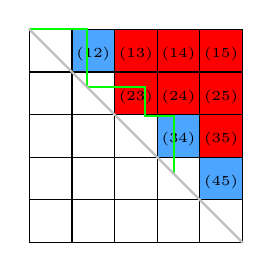
\begin{tikzpicture}[inner sep=0in, outer sep=0in]
                \node (n) {
                \begin{ytableau}
                  \mynone &*(lightblue)\text{\tiny (12)}
                  &*(red)\text{\tiny (13)} &*(red)\text{\tiny (14)}
                  &*(red)
                  \text{\tiny (15)}\\
                  \mynone &\mynone &*(red) \text{\tiny (23)}
                  &*(red)\text{\tiny (24)}
                  &*(red) \text{\tiny (25)}\\
                  \mynone &\mynone &\mynone &*(lightblue) \text{\tiny
                    (34)}
                  &*(red)\text{\tiny (35)} \\
                  \mynone &\mynone &\mynone&\mynone&*(lightblue) \text{\tiny (45)}\\
                  \mynone &\mynone &\mynone&\mynone&\mynone\\
                \end{ytableau}};
              \draw[thick,green] (n.north
              west)--([xshift=2.1em]n.north
              west)--++(0,-2.1em)--++(2.1em,0)--++(0,-1.05em)--++(1.05em,0)--++(0,-2.10em);
              \draw[thick,lightgray] (n.north west)--(n.south east);
              \end{tikzpicture}
              \ \ \
              \scalebox{1.3}{$ 
              \overset{\text{\textcolor{red}{\scriptsize{
                      $\Psi =$ Roots above Dyck
                      path}
                  }
                }}{\text{\textcolor{lightblue}{$\scriptstyle\Delta^+_\ell
                    \setminus \Psi = $ \scriptsize{Non-roots below}}}}
            $}
          \]\pause
          \vspace{-0.1in}
          \begin{block}{Catalan Function~\cite{CH,pany,catalans}}
            For $\Psi$ and $\gamma\in\mathbb Z^\ell$
            $$
            H(\Psi;\gamma)(x) = \prod_{(i,j)\in \textcolor{lightblue}{\Delta^+_\ell
              \setminus \Psi}} (1-R_{ij}) h_\gamma(x)
            $$
          \end{block}\pause
          \begin{itemize}
          \item \(\Psi = \emptyset \implies H(\emptyset;\gamma) =
            s_\gamma\)\pause
          \item \(\Psi =\) all roots \(\implies H(\Psi;\gamma) = h_\gamma\)
          \end{itemize}
        \end{frame}
        \begin{frame}{Catalan functions}
          \begin{block}{\(k\)-Schur root ideal for \(\lambda\)}
            \vspace{-0.1in}
            \begin{align*}
              \Psi = \Delta^k(\lambda)
              & = \{(i,j): j > k-\lambda_i\}\\
              & = \text{root ideal with }k-\lambda_i\text{ \textcolor{lightblue}{non-roots}
                in row }i
            \end{align*}
          \end{block}
          \pause
          \[
            \Delta^4(3,3,2,2,1,1) = 
\ytableausetup{mathmode, boxsize=.8em,centertableaux}
% ~&*(blue!20)&*(red)&*(red)\\
{\scriptsize
\begin{ytableau}
*(white) 3     &*(lightblue)  &*(red)   &*(red)  &*(red)  &*(red) \\
\mynone & *(white)3 & *(lightblue) & *(red) & *(red)  &*(red)  \\
\mynone &*(white)  & *(white)2 & *(lightblue) & *(lightblue)  &*(red)  \\
\mynone &*(white)  & *(white)  & *(white)2 & *(lightblue) &*(lightblue) \\
\mynone &\mynone  &\mynone  &\mynone  & *(white)1 & *(lightblue) \\
\mynone &\mynone  &\mynone  &\mynone  &*(white)  & *(white) 1
\end{ytableau}
}
\quad
\begin{matrix}
\quad
\\
\quad
\\
\leftarrow \text{row $i$ has $4-\lambda_i$ \textcolor{lightblue}{non-roots}}
\\
\quad
\\
\quad
\end{matrix}
\]
\pause
  \begin{block}{\(k\)-Schur is a Catalan function~\cite{catalans}.}
    For partition \(\lambda\) with \(\lambda_1 \leq k\),
    \[s_\lambda^{(k)} = H(\Delta^k(\lambda);\lambda)\,.\]
  \end{block}
\end{frame}
\begin{frame}{Key ingredient of branching proof}
  Dual vertical Pieri rule: \(s_{1^r}^\perp s_\lambda^{(k)} = \sum_\mu
  a_{\lambda \mu} s_\mu^{(k)}\)\,.
  \pause
    \begin{block}{Shift Invariance~\cite{catalans}}
      For partition \(\lambda\) of length \(\ell\) with \(\lambda_1
      \leq k\),
      \[
        s_{1^\ell}^\perp s_{\lambda+1^\ell}^{(k+1)} = s_\lambda^{(k)}
      \]
      where
      \(\langle s_{1^\ell}^\perp f, g \rangle = \langle f, s_{1^\ell}
      g \rangle\).
    \end{block}
    \pause Proof: \(k-\lambda_i = (k+1)-(\lambda_i+1)\)
    \pause
              \[
            \Delta^4(3,3,2,2,1,1) = 
\ytableausetup{mathmode, boxsize=.8em,centertableaux}
% ~&*(blue!20)&*(red)&*(red)\\
{\scriptsize
\begin{ytableau}
*(white) 3     &*(lightblue)  &*(red)   &*(red)  &*(red)  &*(red) \\
\mynone & *(white)3 & *(lightblue) & *(red) & *(red)  &*(red)  \\
\mynone &*(white)  & *(white)2 & *(lightblue) & *(lightblue)  &*(red)  \\
\mynone &*(white)  & *(white)  & *(white)2 & *(lightblue) &*(lightblue) \\
\mynone &\mynone  &\mynone  &\mynone  & *(white)1 & *(lightblue) \\
\mynone &\mynone  &\mynone  &\mynone  &*(white)  & *(white) 1
\end{ytableau}
}
\quad
            \Delta^5(4,4,3,3,2,2) = 
\ytableausetup{mathmode, boxsize=.8em,centertableaux}
% ~&*(blue!20)&*(red)&*(red)\\
{\scriptsize
\begin{ytableau}
*(white) 4     &*(lightblue)  &*(red)   &*(red)  &*(red)  &*(red) \\
\mynone & *(white)4 & *(lightblue) & *(red) & *(red)  &*(red)  \\
\mynone &*(white)  & *(white)3 & *(lightblue) & *(lightblue)  &*(red)  \\
\mynone &*(white)  & *(white)  & *(white)3 & *(lightblue) &*(lightblue) \\
\mynone &\mynone  &\mynone  &\mynone  & *(white)2 & *(lightblue) \\
\mynone &\mynone  &\mynone  &\mynone  &*(white)  & *(white) 2
\end{ytableau}
}
\]
\pause \phantom{Branching is a special case of} Pieri:
\[
      \phantom{s_\lambda^{(k)} =} s_{1^\ell}^\perp s_{\lambda+1^\ell}^{(k+1)} =
      \sum_\mu a_{\lambda+1^\ell, \mu} s_{\mu}^{(k+1)}
    \]
\end{frame}
\begin{frame}{Key ingredient of branching proof}
  Dual vertical Pieri rule: \(s_{1^r}^\perp s_\lambda^{(k)} = \sum_\mu
  a_{\lambda \mu} s_\mu^{(k)}\)\,.
    \begin{block}{Shift Invariance~\cite{catalans}}
      For partition \(\lambda\) of length \(\ell\) with \(\lambda_1
      \leq k\),
      \[
        s_{1^\ell}^\perp s_{\lambda+1^\ell}^{(k+1)} = s_\lambda^{(k)}
      \]
      where
      \(\langle s_{1^\ell}^\perp f, g \rangle = \langle f, s_{1^\ell}
      g \rangle\).
    \end{block}
     Proof: \(k-\lambda_i = (k+1)-(\lambda_i+1)\)

              \[
            \Delta^4(3,3,2,2,1,1) = 
\ytableausetup{mathmode, boxsize=.8em,centertableaux}
% ~&*(blue!20)&*(red)&*(red)\\
{\scriptsize
\begin{ytableau}
*(white) 3     &*(lightblue)  &*(red)   &*(red)  &*(red)  &*(red) \\
\mynone & *(white)3 & *(lightblue) & *(red) & *(red)  &*(red)  \\
\mynone &*(white)  & *(white)2 & *(lightblue) & *(lightblue)  &*(red)  \\
\mynone &*(white)  & *(white)  & *(white)2 & *(lightblue) &*(lightblue) \\
\mynone &\mynone  &\mynone  &\mynone  & *(white)1 & *(lightblue) \\
\mynone &\mynone  &\mynone  &\mynone  &*(white)  & *(white) 1
\end{ytableau}
}
\quad
            \Delta^5(4,4,3,3,2,2) = 
\ytableausetup{mathmode, boxsize=.8em,centertableaux}
% ~&*(blue!20)&*(red)&*(red)\\
{\scriptsize
\begin{ytableau}
*(white) 4     &*(lightblue)  &*(red)   &*(red)  &*(red)  &*(red) \\
\mynone & *(white)4 & *(lightblue) & *(red) & *(red)  &*(red)  \\
\mynone &*(white)  & *(white)3 & *(lightblue) & *(lightblue)  &*(red)  \\
\mynone &*(white)  & *(white)  & *(white)3 & *(lightblue) &*(lightblue) \\
\mynone &\mynone  &\mynone  &\mynone  & *(white)2 & *(lightblue) \\
\mynone &\mynone  &\mynone  &\mynone  &*(white)  & *(white) 2
\end{ytableau}
}
\]
Branching is a special case of Pieri:
\[
      s_\lambda^{(k)} = s_{1^\ell}^\perp s_{\lambda+1^\ell}^{(k+1)} =
      \sum_\mu a_{\lambda+1^\ell, \mu} s_{\mu}^{(k+1)}
    \]
\end{frame}
% \begin{frame}[fragile]{Schubert Calculus Variations}
%       \[
%       \begin{tikzcd}
%         H(\Gr(m,n)) \ar[d] \ar[r]& H(\Gr_{SL_{k+1}}) \ar[d] \\
%         K(\Gr(m,n)) \ar[r] & K(\Gr_{SL_{k+1}})
%       \end{tikzcd}
%     \]
%     \begin{itemize}
%     \item Schubert classes in \(H(\Gr(m,n))\) represented by Schur
%       functions, \(s_\lambda = H(\emptyset;\lambda)\).
%     \item Schubert classes in \(H(\Gr_{SL_{k+1}})\) represented by
%       \(k\)-Schur functions, \(s_\lambda^{(k)} = H(\Delta^k(\lambda);\lambda)\).
%     \item What about \(K\)-theory?
%     \end{itemize}
%   \end{frame}
%   \begin{frame}{Dual Grothendieck polynomials}
%     \begin{itemize}
%     % \item Schubert classes in \(K^*(\Gr(m,n))\) are represented by
%     %   ``Grothendieck polynomials'', denoted \(G_\lambda\).
%     \item Schubert classes in \(K_*(\Gr(m,n))\) are represented by
%       ``dual Grothendieck polynomials'', denoted \(g_\lambda\).
%     \item Let \(k^{(m)}_r = \sum_{i=0}^m \binom{r+i-1}{i} h_{m-i}\)
%       and \(k_\lambda = k^{(0)}_{\lambda_1} \cdots
%       k^{(\ell-1)}_{\lambda_\ell}\) be inhomogeneous analogues of
%       \(h_\lambda\).

%       \ytableausetup{boxsize=0.3em}
%       \(k_{\ydiagram{1,2}} = k_2^{(0)}k_1^{(1)} = h_2(h_1+1) = h_{\ydiagram{1,2}} + h_{\ydiagram{2}} \)

%       \begin{block}{Definition}
%         \(g_\lambda = \prod_{i < j} (1-R_{ij})k_\lambda\)
%       \end{block}
%       \(g_{\ydiagram{1,2}} = s_{\ydiagram{1,2}} + s_{\ydiagram{2}}\)
%     \item Recall Schur function definition \(s_\lambda = \prod_{i < j}
%       (1-R_{ij})h_\lambda\).
%     \end{itemize}
%   \end{frame}
%   \begin{frame}{\(K\)-Theory of Affine Grassmannian}
%   \begin{itemize}
%   \item~\cite{lss} and~\cite{morse} provide equivalent Pieri rules
%     that Schubert representatives \(f_\lambda\) for \(K_*(\Gr_{SL_{k+1}})\) satisfy.
%   \item Call such representatives \(K\)-\(k\)-Schur functions, denoted
%     \(g_\lambda^{(k)}\).
%   \item No direct formulation for \(g_\lambda^{(k)}\).
%   \end{itemize}
%   \begin{block}{Branching Conjecture of~\cite{lss} and~\cite{morse}}
%     \(g_\lambda^{(k)} = \sum_\mu a_{\lambda \mu} g_\mu^{(k+1)}\)
%     satisfies \((-1)^{|\lambda|-|\mu|}a_{\lambda \mu} \in \Z_{\geq 0}\).
%   \end{block}
% \end{frame}
% %
% \begin{frame}{Schubert Calculus Variations}
%   \begin{itemize}
%   \item There are many variations on classical Schubert calculus of the
%   Grassmannian (Type A)%\pause
%   \item (Co)homology of Types BCD Grassmannian, \(K\)-theory of
%     Grassmannian, (Co)homology of affine Grassmannian,\ldots %\pause
%   \begin{block}{Focus}
%     \(K\)-theory and \(K\)-homology of the affine Grassmannian %\pause
%   \end{block}
%   \item Simulatenously generalizes \(K\)-theory of Grassmannian and
%     (co)homology of affine Grassmannian.
%   \end{itemize}
%   % \begin{tabular}{c|p{2.25cm}|p{2.5cm}|p{2.75cm}}
%   %   Cohomology theory
%   %   & Explicit basis
%   %   & Pieri rule
%   %   & LR coefficients \\
%   %   \hline
%   %   Type A
%   %   & Schur
%   %   & Horiz strips
%   %   & Skew Yamanouchi tableaux \\
%   %   \(K\)-theory
%   %   & Grothendieck
%   %   & Set-valued strips
%   %   & Skew set-valued Yamanouchi tableaux \\
%   %   Types BCD
%   %   & Billey-Haiman
%   %   & BH
%   %   & ?? \\
%   %   Quantum
%   %   & ??
%   %   & ??
%   %   & ?? \\
%   %   Affine Type A
%   %   & \(t=1\) \(k\)-Schur 
%   %   & Affine horiz strips
%   %   & Gromov-Witten Invariants?\\
%   %   Affine \(K\)-theory
%   %   & \textcolor{red}{Only indirect}
%   %   & Affine set-valued tableaux
%   %   & Unkown \\
%   %   Affine Type C
%   %   & LSS
%   %   & Unknown
%   %   & Unknown
%   %   \\
%   % \end{tabular}
% \end{frame}
% \begin{frame}{\(K\)-Theory of Affine Grassmannian}
%   \begin{block}{What is known?}
%   %\pause
%     \begin{enumerate}
%     \item \(K\)-theory classes of Grassmannian (not affine!)
%       represented by
%       ``Grothendieck 
%       polynomials.'' We are interested in their dual: \[
%         g_\lambda = \prod_{i < j} (1-R_{ij}) k_\lambda
%       \]
%     \item Homology classes of affine Grassmannian represented by
%       \(k\)-Schur functions (\(t=1\)) \[
%         s_\lambda^{(k)} = \prod_{(i,j) \in \Delta^+_\ell \setminus
%           \Delta^{(k)}(\lambda)} (1-R_{ij}) h_\lambda
%         \] %\pause
%         \vspace{-0.2in}
%      \item Is there a common generalization of these formulas?
% %    \item~\cite{lss} leave open the question: what is a direct formulation of the \(K\)-homology representatives of the affine Grassmannian (\(K\)-\(k\)-Schur functions)?
%     \end{enumerate}
%   \end{block}
% \end{frame}
\begin{frame}{Overview}
  \begin{itemize}
  \item Schubert calculus
  \item Catalan functions: a new approach to old problems
  \item \textbf{\(K\)-theoretic Catalan functions}
  \end{itemize}
\end{frame}
\begin{frame}{Dual Grothendieck polynomials}
  \begin{itemize}
  \item Inhomogeneous basis: \(g_\lambda = s_\lambda +\) lower degree terms.\pause
  \item Satisfies Pieri rule on ``set-valued strips''
    \ytableausetup{aligntableaux=bottom,boxsize=0.4em} \pause
    \begin{align*}
      g_{1^2} g_{3,2} = 
      & g_{43}
      + g_{421}
      + g_{331}
      - g_{42}
      - g_{33}
      -2 g_{321}
      + g_{31}\\
      & \ydiagram{2,3}*[*(red)]{2+1,3+1}\quad
      \ydiagram{0,2,3}*[*(red)]{1,0,3+1}\quad
      \ydiagram{0,2,3}*[*(red)]{1,2+1}\quad
      \ydiagram{2,3}*[*(red)]{0,3+1}*[*(lightgray)]{1+1}\quad
      \ydiagram{2,3}*[*(red)]{2+1}*[*(lightgray)]{0,2+1}\quad
      \ydiagram{0,2,3}*[*(red)]{1}*[*(lightgray)]{0,1+1}\,
      \ydiagram{0,2,3}*[*(red)]{1}*[*(lightgray)]{0,0,2+1}\quad
      \ydiagram{2,3}*[*(lightgray)]{1+1,2+1}
    \end{align*}\pause
    \item \(g_\lambda = \prod_{i < j} (1-R_{ij}) k_\lambda\) for
      \(k_\lambda\) and inhomogeneous analogue of \(h_\lambda\).\pause
    \item Dual to Grothendieck polynomials \(G_\lambda\): Schubert representatives
      for \(K^*(Gr(m,n))\)
  \end{itemize}
\end{frame}
\begin{frame}{\(K\)-\(k\)-Schur functions}
  \begin{itemize}
  \item Inhomogeneous basis: \(g_\lambda^{(k)} = s_\lambda^{(k)} +
    \)lower degree terms \pause
  \item Satisfies Pieri rule on ``affine set-valued strips''\pause
    \ytableausetup{centertableaux,boxsize=1.0em}
    \begin{align*}
      g_1 g_{211}^{(2)} & = g_{2111}^{(2)} -
      2g_{211}^{(2)} \quad\quad\quad \text{\scriptsize $2$-bounded partitions $\correspondsto$ $3$-cores}\\
      \begin{ytableau}
        \none[\textcolor{red}{\bullet}] &
        \none[\textcolor{blue}{\bullet}] &
        \none[\textcolor{black}{\bullet}] &
        \none[\textcolor{red}{\bullet}] &
        \none[\textcolor{blue}{\bullet}] \\
        \textcolor{blue}{\bullet} &
        \none[\textcolor{black}{\bullet}] &
        \none[\textcolor{red}{\bullet}] &
        \none[\textcolor{blue}{\bullet}] &
        \none[\textcolor{black}{\bullet}] \\
        \textcolor{black}{\bullet} &
        \none[\textcolor{red}{\bullet}] &
        \none[\textcolor{blue}{\bullet}] &
        \none[\textcolor{black}{\bullet}] &
        \none[\textcolor{red}{\bullet}] \\
        \textcolor{red}{\bullet} &
        \textcolor{blue}{\bullet} &
        \textcolor{black}{\bullet} &
        \none[\textcolor{red}{\bullet}] &
        \none[\textcolor{blue}{\bullet}]
      \end{ytableau}&\to
      \begin{ytableau}
        *(lightgray) \textcolor{red}{\bullet} &
        \none[\textcolor{blue}{\bullet}] &
        \none[\textcolor{black}{\bullet}] &
        \none[\textcolor{red}{\bullet}] &
        \none[\textcolor{blue}{\bullet}] \\
        \textcolor{blue}{\bullet} &
        \none[\textcolor{black}{\bullet}] &
        \none[\textcolor{red}{\bullet}] &
        \none[\textcolor{blue}{\bullet}] &
        \none[\textcolor{black}{\bullet}] \\
        \textcolor{black}{\bullet} &
        *(lightgray) \textcolor{red}{\bullet} &
        \none[\textcolor{blue}{\bullet}] &
        \none[\textcolor{black}{\bullet}] &
        \none[\textcolor{red}{\bullet}] \\
        \textcolor{red}{\bullet} &
        \textcolor{blue}{\bullet} &
        \textcolor{black}{\bullet} &
        *(lightgray) \textcolor{red}{\bullet} &
        \none[\textcolor{blue}{\bullet}]
      \end{ytableau}-
      \begin{ytableau}
        \none[\textcolor{red}{\bullet}] &
        \none[\textcolor{blue}{\bullet}] &
        \none[\textcolor{black}{\bullet}] &
        \none[\textcolor{red}{\bullet}] &
        \none[\textcolor{blue}{\bullet}] \\
        *(lightgray) \textcolor{blue}{\bullet} &
        \none[\textcolor{black}{\bullet}] &
        \none[\textcolor{red}{\bullet}] &
        \none[\textcolor{blue}{\bullet}] &
        \none[\textcolor{black}{\bullet}] \\
        \textcolor{black}{\bullet} &
        \none[\textcolor{red}{\bullet}] &
        \none[\textcolor{blue}{\bullet}] &
        \none[\textcolor{black}{\bullet}] &
        \none[\textcolor{red}{\bullet}] \\
        \textcolor{red}{\bullet} &
        \textcolor{blue}{\bullet} &
        \textcolor{black}{\bullet} &
        \none[\textcolor{red}{\bullet}] &
        \none[\textcolor{blue}{\bullet}]
      \end{ytableau}-
      \begin{ytableau}
        \none[\textcolor{red}{\bullet}] &
        \none[\textcolor{blue}{\bullet}] &
        \none[\textcolor{black}{\bullet}] &
        \none[\textcolor{red}{\bullet}] &
        \none[\textcolor{blue}{\bullet}] \\
        \textcolor{blue}{\bullet} &
        \none[\textcolor{black}{\bullet}] &
        \none[\textcolor{red}{\bullet}] &
        \none[\textcolor{blue}{\bullet}] &
        \none[\textcolor{black}{\bullet}] \\
        \textcolor{black}{\bullet} &
        \none[\textcolor{red}{\bullet}] &
        \none[\textcolor{blue}{\bullet}] &
        \none[\textcolor{black}{\bullet}] &
        \none[\textcolor{red}{\bullet}] \\
        \textcolor{red}{\bullet} &
        \textcolor{blue}{\bullet} &
        *(lightgray) \textcolor{black}{\bullet} &
        \none[\textcolor{red}{\bullet}] &
        \none[\textcolor{blue}{\bullet}]
      \end{ytableau}
    \end{align*}\pause
  \item Conjecture: \(g_\lambda^{(k)}\) have positive branching into
    \(g_\mu^{(k+1)}\)~\cite{lss,morse}.\pause
    \begin{block}{Problem}
      No direct formula for \(g_\lambda^{(k)}\)
    \end{block}
  \end{itemize}
\end{frame}
\begin{frame}{An Extra Ingredient: Lowering Operators}
   Lowering Operators 
     \(L_j(f_\lambda) = f_{\lambda-\epsilon_j}\)
            \ytableausetup{boxsize=1.0em,centertableaux}
            \[ L_3\left( \ydiagram{1,1,3}*[*(red)]{1} \right) =
              \ydiagram{1,3}, \ \ L_{1}\left( \ydiagram{1,1,3}*[*(red)]{0,0,2+1} \right)
              = \ydiagram{1,1,2}
              \]
  % \item Root ideal \(\Psi\): given by Dyck path.
  %           \ytableausetup{mathmode, boxsize=1em,centertableaux}
  %           \[
  %             \Psi =
  %             \begin{ytableau}
  %               \mynone &*(lightblue)\text{\tiny (12)}  &*(red)\text{\tiny (13)}   &*(red)\text{\tiny (14)}  &*(red)
  %               \text{\tiny (15)}\\
  %               \mynone &\mynone &*(red) \text{\tiny (23)}  &*(red)\text{\tiny (24)}
  %               &*(red) \text{\tiny (25)}\\
  %               \mynone &\mynone &\mynone &*(lightblue) \text{\tiny (34)}
  %               &*(red)\text{\tiny (35)} \\
  %               \mynone &\mynone &\mynone&\mynone&*(lightblue) \text{\tiny (45)}\\
  %               \mynone &\mynone &\mynone&\mynone&\mynone\\
  %             \end{ytableau}
  %             \ \ \ \overset{\text{\textcolor{red}{\scriptsize{Roots above Dyck
  %                   path}}}}{\text{\textcolor{blue}{\scriptsize{Non-roots below}}}}
  %           \] 
\end{frame}
\begin{frame}{Affine \(K\)-Theory Representatives with Raising Operators}
  \begin{block}{\(K\)-theoretic Catalan function}
    Let \(\Psi,\lowers \subset \Delta^+_\ell\) be order ideals of
    positive roots and \(\gamma \in \Z^\ell\), then
    \[
      K(\Psi;\lowers;\gamma) := \prod_{(i,j) \in \lowers} (1-L_j)
      \prod_{(i,j) \in \Delta^+_\ell \setminus \Psi} (1-R_{ij})
      k_\gamma
    \]\pause
  \end{block}
  \begin{example}
    \(\textcolor{lightblue}{\text{non-roots of }\Psi},
              \textcolor{coralred}{\text{roots of }\lowers}\)
              \begin{columns}
                \begin{column}{0.20\textwidth}
                  \ytableausetup{mathmode,
                    boxsize=1em,centertableaux} \[
                    \begin{ytableau}
                      \mynone &*(lightblue)\text{\tiny (12)}
                      &*(white)\text{\tiny (13)}
                      &*(coralred)\text{\tiny (14)} &*(coralred)
                      \text{\tiny (15)}\\
                      \mynone &\mynone &*(white) \text{\tiny (23)}
                      &*(coralred)\text{\tiny (24)}
                      &*(coralred) \text{\tiny (25)}\\
                      \mynone &\mynone &\mynone &*(lightblue)
                      \text{\tiny (34)}
                      &*(white)\text{\tiny (35)} \\
                      \mynone &\mynone &\mynone&\mynone&*(lightblue) \text{\tiny (45)}\\
                      \mynone &\mynone &\mynone&\mynone&\mynone\\
                    \end{ytableau}
                  \]
                \end{column}
                \begin{column}{0.80\textwidth}
                  \begin{align*}
                    & K(\Psi;\lowers;54332) \\
                    & = \textcolor{coralred}{(1-L_{4})^2(1-L_{5})^2} \textcolor{lightblue}{(1-R_{12})(1-R_{34})(1-R_{45})} k_{54332}
                  \end{align*}
                \end{column}
              \end{columns}
            \end{example}
\end{frame}
% \begin{frame}{Affine \(K\)-Theory Representatives with Raising
%     Operators}
%   \begin{definition}
%     The \emph{\(k\)-Schur root ideal}, \(\Delta^{(k)}(\lambda)\) is the
%     unique root ideal with \(\lambda_i + \#\)non-roots in row \(i =
%     k\).
%   \end{definition}
%   \begin{example}
%   \(k=4, \lambda = 332111\)
%               \[
%               \Delta^{(4)}(332111) = 
%               {\footnotesize
%                 \begin{ytableau}
%                   *(white) 3     &*(lightblue)  &*(red)   &*(red)  &*(red)  &*(red) \\
%                   \mynone & *(white)3 & *(lightblue) & *(red) & *(red)  &*(red)  \\
%                   \mynone & \mynone  & *(white)2 & *(lightblue) & *(lightblue)  &*(red)  \\
%                   \mynone & \mynone  & \mynone  & *(white)1 & *(lightblue) &*(lightblue) \\
%                   \mynone &\mynone  &\mynone  &\mynone  & *(white)1 & *(lightblue) \\
%                   \mynone &\mynone  &\mynone  &\mynone  & \mynone  & *(white) 1
%                 \end{ytableau}
%               }
%               \leftarrow\,\text{\small{4 - 2 non-roots}}
%               \quad
%             \]
%             \end{example}
% \end{frame}
\begin{frame}{Affine \(K\)-Theory Representatives with Raising Operators}
  \begin{block}{Answer (Blasiak-Morse-S., 2020)}
    \pause
    For \(K\)-homology of affine Grassmannian, \(g_\lambda^{(k)} =
    K(\Delta^{k}(\lambda); \Delta^{k+1}(\lambda);\lambda)\) since this family satisfies the Pieri rule. 
  \end{block}
  \pause
  \begin{example}
\(              g_{332111111}^{(4)} = \){\footnotesize
                \begin{ytableau}
                  *(white) 3     &*(lightblue)  &*(white)
                  &*(coralred)  &*(coralred)  &*(coralred) &
                  *(coralred) & *(coralred) & *(coralred)\\
                  \mynone & *(white)3 & *(lightblue) & *(white) &
                  *(coralred)  &*(coralred) & *(coralred) &
                  *(coralred) & *(coralred)\\
                  \mynone &\mynone  & *(white)2 & *(lightblue) &
                  *(lightblue)  &*(white) &*(coralred) & *(coralred) &
                  *(coralred)\\
                  \mynone &\mynone  & \mynone  & *(white)1 &
                  *(lightblue) &*(lightblue) & *(lightblue) & *(white)
                  & *(coralred)\\
                  \mynone &\mynone  &\mynone  &\mynone  & *(white)1 &
                  *(lightblue) & *(lightblue) & *(lightblue) & *(white) \\
                  \mynone &\mynone  &\mynone  &\mynone  &\mynone &
                  *(white) 1 & *(lightblue) & *(lightblue) & *(lightblue)\\
                  \mynone &\mynone  &\mynone  &\mynone  &\mynone &
                  \mynone & *(white) 1 & *(lightblue) & *(lightblue)\\
                  \mynone &\mynone  &\mynone  &\mynone  &\mynone &
                  \mynone & \mynone & *(white) 1 & *(lightblue) \\
                  \mynone &\mynone  &\mynone  &\mynone  &\mynone &
                  \mynone & \mynone & \mynone & *(white) 1
                \end{ytableau}
              }
\hspace{0.25in}\(\textcolor{lightblue}{\Delta^+_9 / \Delta^{4}(332111111)}, \textcolor{coralred}{\Delta^{5}(332111111)}\)
\end{example}
\end{frame}
% \begin{frame}[fragile]{Unified Description of Schubert Representative}
%   \[
%     \begin{tikzcd}
%     H(\Gr(m,n)) \ar[d] \ar[r]& H(\Gr_{SL_{k+1}}) \ar[d] \\
%     K(\Gr(m,n)) \ar[r] & K(\Gr_{SL_{k+1}})
%     \end{tikzcd}
%   \]
%   Schubert representatives \(f_\lambda\) for
%   \begin{itemize}
%   \item \(H_*(\Gr(m,n))\) are \(s_\lambda = H(\emptyset;\lambda)\).
%   \item \(H_*(\Gr_{SL_{k+1}})\) are \(s_\lambda^{(k)} =
%     H(\Delta^k(\lambda);\lambda)\).
%   \item \(K_*(\Gr(m,n))\) are \(g_\lambda =
%     K(\emptyset;\emptyset;\lambda)\).
%   \item \(K_*(\Gr_{SL_{k+1}})\) are \(g_\lambda^{(k)} = K(\Delta^k(\lambda);\Delta^{k+1}(\lambda);\lambda)\).
%   \end{itemize}
% \end{frame}
\begin{frame}{Branching Positivity}
  \begin{theorem}[Blasiak-Morse-S., 2020]
    \pause
    The \(g_\lambda^{(k)}\) are ``shift
        invariant'', i.e.\,for \(\ell = \ell(\lambda)\)
      \[
        G_{1^\ell}^\perp g_{\lambda+1^\ell}^{(k+1)} = g_\lambda^{(k)}
      \]
  \end{theorem}\pause
  \begin{theorem}[Blasiak-Morse-S., 2020]
    The branching coefficients in 
    \[
      g_\lambda^{(k)} = \sum_\mu a_{\lambda \mu} g_\mu^{(k+1)}
    \]
    satisfy \((-1)^{|\lambda|-|\mu|}a_{\lambda \mu} \in \Z_{\geq 0}\).
  \end{theorem}
\end{frame}
\begin{frame}{\(K\)-theoretic Peterson isomorphism}
  \vspace{-0.2in}
   \[
    \Phi \colon QK^*(Fl_{k+1}) \to K_*(Gr_{SL_{k+1}})_{loc}
  \]
  \pause
  \vspace{-0.2in}
  \begin{block}{Conjecture~\cite{IIM}}
    For \(w \in S_{k+1}\) and \(\G_w^Q\) a ``quantum Grothtendieck
    polynomial'',
    \vspace{-0.1in}
    \[
      \Phi(\G_w^Q) = \frac{\tilde{g}_w}{\prod_{i \in Des(w)} \tau_i}
    \]

    \pause
    satisfies \(\tilde{g}_w = g_\lambda^{(k)} + \sum_\mu a_{\lambda
      \mu} g_\mu^{(k)}\) such that \((-1)^{|\lambda|-|\mu|}a_{\lambda
      \mu} \in \Z_{\geq 0}\).
  \end{block}\pause
  \setbeamercolor{block title}{use=structure,fg=white,bg=green!40!black}
  \setbeamercolor{block body}{use=structure,fg=black,bg=lime!10!white}
  \begin{theorem}[Blasiak-Morse-S., 2020]
    If \(\lambda \subset (d^{k+1-d})\) for some \(1 \leq d \leq k\),
    then \(g_\lambda^{(k)} = g_\lambda\). Thus, conjecture is true
    for \(w\) a Grassmannian permutation (i.e. \(w\) has only one descent).
  \end{theorem}\pause
  \begin{block}{Conjecture (Blasiak-Morse-S., 2020)}
    \[\tilde{g}_w = K(\Delta^k(\lambda);\Delta^k(\lambda);\lambda)\]
  \end{block}
\end{frame}
\begin{frame}{Future Directions}
    For \(G_\lambda^{(k)}\) an affine Grothendieck polynomial (dual to \(g_\lambda^{(k)}\)),\pause
    \begin{enumerate}
    \item Combinatorially describe dual Pieri rule: \(G_{1^r}^\perp g_\lambda^{(k)} = \sum_\mu
      ?? g_\mu^{(k)} \iff G_{1^r} G_\mu^{(k)} = \sum_\lambda ?? G_\lambda^{(k)}\),  \(1 \leq r \leq k\).\pause
    \item Combinatorially describe branching coefficients: \(g_\lambda^{(k)} =
      \sum_\mu ?? g_\mu^{(k+1)}\).\pause
    \item Combinatorially describe \(g_\lambda^{(k)} = \sum_\mu ??
      s_\mu^{(k)}\).\pause
    \item Prove the image of \(\G_w^Q\) under \(K\)-theoretic Peterson isomorphism
      for all \(w \in S_{k+1}\).
    \end{enumerate}
\end{frame}
\begin{frame}[shrink=10]{References}
  \textbf{Thank you!}
  \begin{bibdiv}
    \begin{biblist}
    \bib{act}{article}{
      author={Anderson, David}
      author={Chen, Linda}
      author={Tseng, Hsian-Hua}
      title={On the quantum \(K\)-ring of the flag manifold}
      year={2017}
      status={preprint}
      note={arXiv: 1711.08414}
    }
    \bib{catalans}{article}{
      author={Blasiak, Jonah}
      author={Morse, Jennifer}
      author={Pun, Anna}
      author={Summers, Daniel}
      title={Catalan Functions and \(k\)-Schur Positivity}
      year={2019}
      journal={J. Amer. Math. Soc.}
      volume={32}
      number={4}
      pages={921--963}
    }
    \bib{CH}{thesis}{
      author={Chen, Li-Chung}
      title={Skew-linked partitions and a representation theoretic
        model for \(k\)-Schur functions}
      type={Ph.D. thesis}
      year={2010}
      ios={U.C. Berkeley}
    }
    \bib{IIM}{article}{
      author={Ikeda, Takeshi}
      author={Iwao, Shinsuke}
      author={Maeno, Toshiaki}
      title={Peterson Isomorphism in \(K\)-theory and Relativistic
        Toda Lattice}
      status={preprint}
      year={2018}
      note={arXiv: 1703.08664}
    }
    \bib{Lam08}{article}{
      author={Lam, Thomas}
      title={Schubert polynomials for the affine Grassmannian}
      journal={J. Amer. Math. Soc.}
      volume={21}
      year={2008}
      number={1}
      pages={259--281}
    }
    \bib{llms}{article}{
      author={Lam, Thomas}
      author={Lapointe, Luc}
      author={Morse, Jennifer}
      author={Shimozono, Mark}
      title={Affine insertion and Pieri rules for the affine
        Grassmannian}
      journal={Mem. Amer. Math. Soc.}
      volume={208}
      year={2010}
      number={977}
    }
    \bib{lss}{article}{
      author={Lam, Thomas}
      author={Schilling, Anne}
      author={Shimozono, Mark}
      title={K-theory Schubert calculus of the affine
        Grassmannian}
      year={2010}
      journal={Compositio Math.}
      volume={146}
      pages={811--852}
    }
    \bib{lapointe-lascoux-morse}{article}{
      author={Lapointe, Luc}
      author={Lascoux, Alain}
      author={Morse, Jennifer}
      title={Tableau atoms and a new Macdonald positivity conjecture}
      journal={Duke Mathematical Journal}
      year={2003}
      volume={116}
      number={1}
      pages={103--146}
    }
    \bib{morse}{article}{
      author={Morse, Jennifer}
      title={Combinatorics of the K-theory of affine
        Grassmannians}
      year={2011}
      journal={Advances in Mathematics}
    }
    \bib{pany}{article}{
      author={Panyushev, Dmitri I.}
      title={Generalised Kostka-Foulkes polynomials and cohomology of
        line bundles on homogeneous vector bundles}
      journal={Selecta Math. (N.S.)}
      volume={16}
      year={2010}
      number={2}
      pages={315--342}
    }
  \end{biblist}
\end{bibdiv}
\end{frame}
\end{document}